\documentclass{memoir}

%\usepackage{fancyhdr}
\usepackage{xcolor}
\usepackage{hyperref}
\usepackage{graphicx}
\usepackage{enumitem}
\usepackage{verbatim}

\graphicspath{{../figures/}}
\hypersetup{
  colorlinks,
  linkcolor={red!50!black},
  citecolor={blue!50!black},
  urlcolor={blue!80!black}
}
\urlstyle{same}
\setlength{\headheight}{15.2pt}
\pagestyle{simple}
%\fancyhf{}
%\lfoot[$\the\numexpr\value{page}$]{} %-1 to take into account title page.
%\rfoot[]{$\the\numexpr\value{page}$}

\begin{document}

\chapter{Introduction}
\label{chap:introduction}

\chapter{Preparations}
\label{chap:preparations}

\section{Data sets}
\label{sec:datasets}


\subsection{Other notes}
\label{sec:othernotesdatasets}

The program is not able to read csv-files that have so-called newline symbols (\textbackslash n) or carriage return symbols (\textbackslash r) in their text cells. The reason for this is that the program uses a relatively simple csv-file parser, which will think that a new line of data will start after encountering one of these symbols (each line of data in a csv-file will end with a newline symbol by default). The program is typically able to recognise when an 'illegal' newline is encountered, and it will throw an error (see figure \ref{fig:importerror}). Solving the error is left to the user. The problem can be solved by removing all newline symbols and carriage return symbols from the csv-file with the dataset. These symbols are not visible in programs like Excel or LibreOffice Calc, and in both programs you will need to use special search and replace options to get rid of the unwanted symbols. I advise you to Google for ``Find and replace regular expressions with [your spreadsheet program]''. 

\chapter{Using the program}
\label{chap:usingtheprogram}

\section{Loading a new dataset}
\label{sec:loadingnewdataset}

Importing the new data into the program works as follows. You first need to select the csv-file containing your data. For this you will click the \textbf{Select File} button (see figure \ref{fig:importoptions}), which will open a file dialog that you can use to navigate to, and select the file.

Once a file has been selected, you will need to select the delimiter symbol that is used in the csv-file to distinguish between different columns of the data table. For this, you can use the dropdown menu that reads \textbf{-Select delimiter-} by default. Four different symbols are allowed as delimiter, which are the comma (,), the semicolon (;), the colon (:), and the vertical bar (\textbar). Make sure that the delimiter that you select matches the one used in the file.

Once you have selected a delimiter, you can import the data, using the \textbf{Import data} button. Once you click this button, the program will attempt to read data from selected file and, if successful, enable all other options of the program, allowing you to start coding.   

\begin{figure}[h!]
  \centering
  \caption{Options to import data.}
  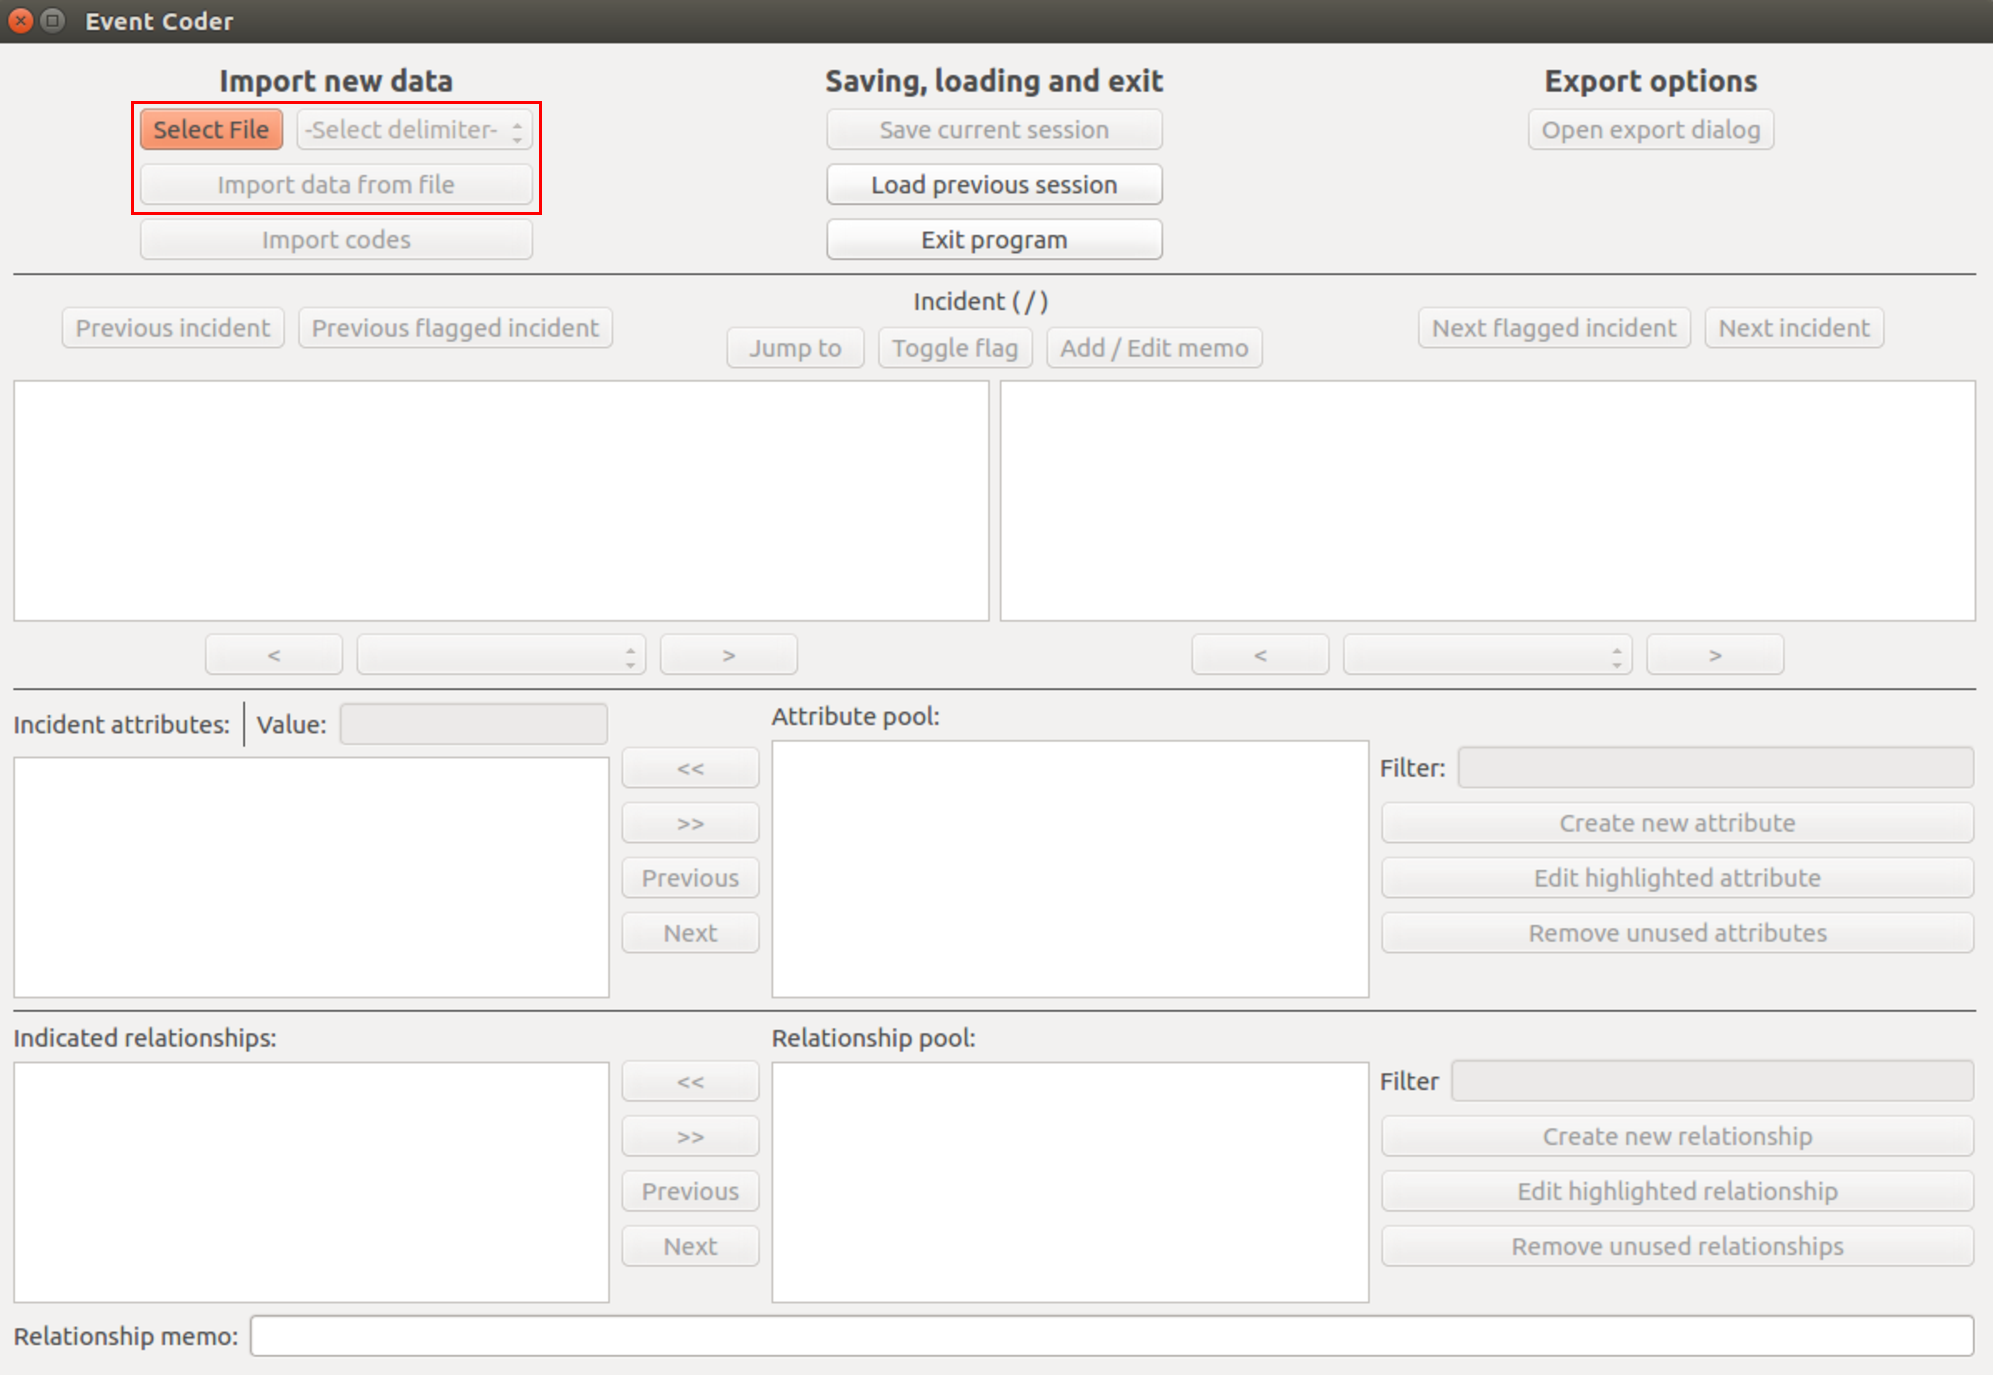
\includegraphics[width=80mm]{Screenshot_0.pdf}
  \label{fig:importoptions}
\end{figure}

\subsection{Problems when importing data}
\label{sec:importerrors}

If you (1) selected a valid csv-file, (2) selected the correct delimiter for this file, and (3) structured your data set using instructions offered in section \ref{sec:datasets}, you should encounter no problems when importing the data. If something goes wrong when importing data, then the problem will usually lie with one of these three points.

One possibility is that you have not selected a valid csv-file. I have encountered a few people that have tried to create csv-files from (for example) xls-files by simply changing the file extension. Doing this will not actually create a valid csv-file that can be read by the program. The correct way for creating csv-files is to use the \textbf{Save as} option in your spreadsheet editor, and select to save the file with the \textbf{*.csv} extension.

If you selected the wrong delimiter, the program will usually import the data, but it will fail to distinguish between different columns of the data set, and possibly assume that the entire dataset only contains one column. This should be obvious from the texts displayed by the program. In this case, simply import the data again, using the correct delimiter. 

If you see the error message displayed in figure \ref{fig:importerror}, this means that some cells of your data set probably contain newline symbols and/or carriage return symbols that need to be removed before importing data (see section \ref{sec:othernotesdatasets}).

\begin{figure}[h!]
  \centering
  \caption{Data import error report.}
  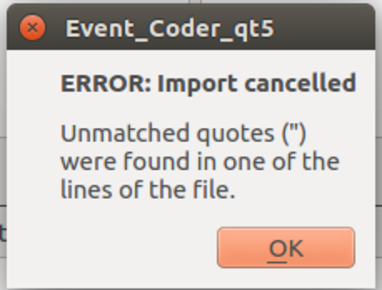
\includegraphics[width=40mm]{Screenshot_1.pdf}
  \label{fig:importerror}
\end{figure}

If you are certain that you made no mistakes in one of these points, and you still encounter problems when importing your data set, then you may have encountered a bug in the program that needs to be fixed. In that case, please get in touch with me (see chapter \ref{chap:contactdetails}).


\chapter{Contact details}
\label{chap:contactdetails}





\end{document}